% !TEX root = ../Vorlage_DA.tex
%	########################################################
% 				Aufgabenstellung/Pflichtenheft
%	########################################################


%	--------------------------------------------------------
% 	Überschrift, Inhaltsverzeichnis
%	--------------------------------------------------------
\chapter{Konzept}

%	--------------------------------------------------------
% 	Grundlegende Idee
%	--------------------------------------------------------
    \section{Grundlegende Idee}\label{ref:Konzept}
    
        sunnyHOME sollte eine Wetterstation werden, welche für jeden Hobby-Elektroniker leicht zu bedienen und zu konfigurieren ist. Man sollte sie einfach in den Wald stellen können, ohne sich jegliche Sorgen um Stromversorgung machen zu müssen. Das heißt sie sollte Energie-autark werden. 
        
        \begin{figure}[H]
            \centering
            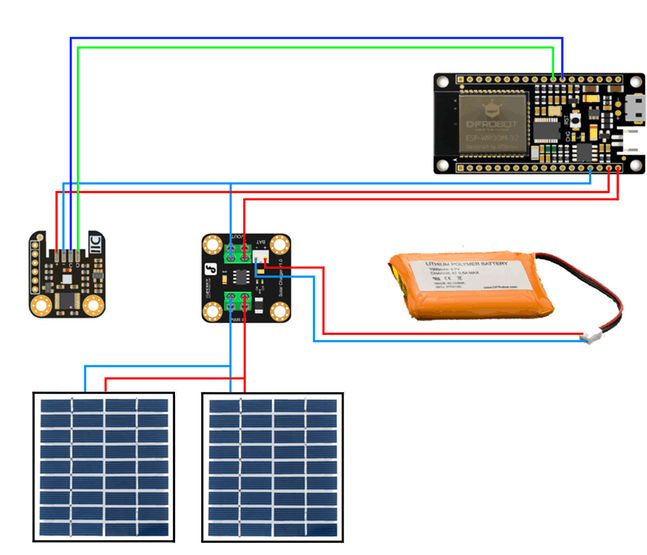
\includegraphics[width=0.5\textwidth]{./media/images/Schema.png}
            \caption{Aufbau der Wetterstation.\cite{bib:HugoGomes}}
            \label{fig:Aufbau}
        \end{figure}
        
        Ebenfalls sollte eine Funkverbindung implementiert werden. Dies wäre nötig, um eine Kommunikation über mehrere Kilometer gewährleisten zu können. 
        
        In einem weiteren Schritt sollte eine intuitive Website und App programmiert werden. Über diese sollte man dann die empfangenen Sensordaten auslesen, und den Standort der Wetterstation abrufen können. 
        
        
%	--------------------------------------------------------
% 	Kommunikation
%	--------------------------------------------------------
    \section{Kommunikation}
    
         Ein ESP32 (siehe: \ref{ref:ESP32}) hat standardmäßig WLAN und Bluetooth verbaut. Ein Ziel des Projektes war jedoch, die Positionierung der Wetterstation, weit weg von jeglichen WLAN-Netzen und Bluetooth-Receivern zu positionieren. Um dies zu verwirklichen war zuerst ein Funk-Modul vorgesehen. 
         Im späteren Laufe des Projektes, wurde die Kommunikation über WLAN vorgezogen, da diese keine zusätzliche Hardware für einen MQTT-Broker braucht, und Zeit aufgeholt werden musste.
        
\pagebreak
        
%	--------------------------------------------------------
% 	Energie-Management
%	--------------------------------------------------------
    \section{Energie-Management}
    
         Für die Energie-Versorgung ist eine 9V-Solarzelle beschaffen worden. Diese wurde anderen Solarzellen vorgezogen, weil sei eine bessere „Low-Light Performance“ bietet. Da sie eine höhere Spannung liefert, können kleinere Ströme wahrgenommen werden, welche dann über ein Energy-Harvesting Modul den Akku speisen.
        
        \begin{figure}[H]
            \centering
            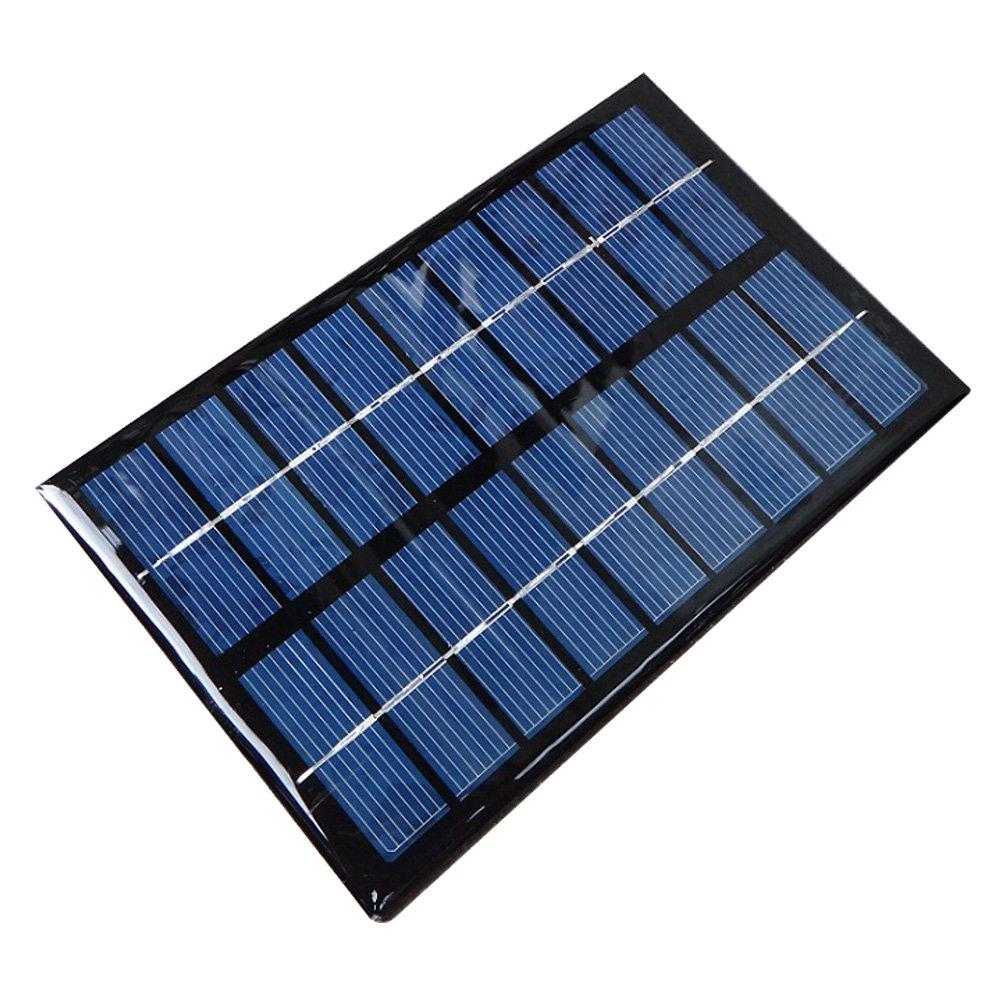
\includegraphics[width=0.3\textwidth]{./media/images/SolarPanel.jpg}
            \caption{9V Solarzelle \cite{bib:SolarPanel}}
            \label{fig:SolarPanel}
        \end{figure}
        
        Energy-Harvesting Module können wie Kondensatoren verstanden werden. Sie werden mit niedrigen Strömen aufgeladen, und wenn sie sich dann aufgeladen haben, wird der ganze Strom mit einen Schub in den Akku gespeist. Nötig ist das, da Akkus keine zu niedrigen Ströme aufnehmen können. 
        
        Um zusätzlich an Energie zu sparen, gibt es beim ESP32 verschiedene \textbf{„Power-Modes“}: 
        
        \begin{itemize}
            \item \textbf{Active Mode: }        Der Chip ist voll funktionstüchtig. Er kann Empfangen, Versenden und Zuhören
            \item \textbf{Modem-Sleep Mode: }	Der CPU ist betriebsbereit und der Takt lässt sich konfigurieren. Funkverbindungen sind ausgeschalten
            \item \textbf{Light-Sleep Mode: }	Der CPU ist pausiert. Der RTC-Speicher und die RTC-Peripherien (RTC ... Real-Time Clock), sowie der ULP Co-Prozessor (ULP ... Ultra-Low-Power) sind am Laufen. Verschiedene Wake-Up Events können das Aufwachen des Chips verursachen. 
            \item\label{ref:DeepSleep} \textbf{Deep-Sleep Mode: }    Nur der RTC-Speicher und die RTC-Peripherien sind eingeschalten. Verbindungsdaten sind im RTC-Speicher gespeichert. ULP Co-Prozessor ist funktionsbereit. 
            \item \textbf{Hibernation Mode: }   Der interne 8MHz Oszillator und der ULP Co-Prozessor sind ausgeschalten. Nur der RTC-Timer am langsamen Tackt und einige RTC GPIOs sind aktiv. Der RTC-Timer oder die RTC-GPIOs können den Chip aus dem Hibernation Mode aufwecken. 
        \end{itemize}
        \begin{flushright}
            \cite{bib:esp32datasheet}
        \end{flushright}
        Im Programm wurde der Deep-Sleep Mode gewählt. Es kann ein Intervall eingestellt werden, in dem der ESP immer hochfährt, die Daten sendet, und dann wieder in den Schlaf-Modus zurückkehrt. 
        
\pagebreak

         
%	--------------------------------------------------------
% 	Visualisierung
%	--------------------------------------------------------
    \section{Visualisierung}
    
         Wie bereits in \ref{ref:Konzept} erwähnt, sollte eine App und eine Website realisiert werden. Hauptanliegen dieser Applikationen waren: 
         
         \begin{itemize}
            \item   eine umfassende Übersicht über gemessene Sensordaten
            \item   das Tracken der Wetterstation
            \item   eine intuitive, benutzerfreundliche Oberfläche
            \item   die Möglichkeit Einstellungen des ESP zu verwalten
        \end{itemize}
        
        Um das Pensum des Projektes zu kürzen, musste auf die Entwicklung von eigenen Applikationen verzichtet werden. Dafür wurde ein online MQTT-Broker implementiert, welcher es möglich macht, alle obigen Punkte zu realisieren (siehe: \ref{ref:Ubidots}).
        
         
%	--------------------------------------------------------
% 	Funktionsablauf
%	--------------------------------------------------------
    \section{Funktionsablauf} \label{ref:FnktAb}
    
        Für den Funktionsablauf des Programms wurde eine Struktur festgelegt. In der folgenden Abbildung \ref{fig:FnktAb} sieht man, nach welcher Reihenfolge die Teilaufgaben des Programms geordnet sind. 
    
         \begin{figure}[H]
            \centering
            
\includegraphics[width=1\textwidth]{./media/images/FnktAb.jpg}
            \caption{Illustration zum Funktionsablauf}
            \label{fig:FnktAb}
        \end{figure}
        
        Sobald der Controller aus dem Deep-Sleep Mode (siehe: \ref{ref:DeepSleep}) aufwacht, soll versucht werden, eine Verbindung zum Internet und zum MQTT-Broker aufzubauen. Ist dies geschehen, wird auf GPS-Daten Empfang gewartet. Sobald sie dann empfangen werden, wird die RTC mit der GPS-Zeit synchronisiert. Danach erfolgen die Sensor-Messungen, welche im nächsten Schritt, zusammen mit den GPS-Daten, an den MQTT-Broker versendet werden sollen. Ist die Routine zu Ende, wird der Deep-Sleep Modus wieder gestartet, und der Timer gestellt, nachdem der Controller wieder aufwachen soll.  
         
